% LaTeX .tex
% Example for the proceedings of the  25th International Congress of Mechanical Engineering
% COBEM 2019
% October, 20-25, 2019, Uberlândia, MG, Brazil
% Based on the template of the proceedings of COBEM2015 and COBEM2017

\documentclass[10pt,fleqn,a4paper,twoside]{article}
\usepackage{abcm}
\def\shortauthor{F. J. O. Ribeiro, I. A. Macedo, A. Z. Guarato, R. L. R. Neves}
\def\shorttitle{Development and Validation of Winding Machine}
\usepackage{blindtext}
\usepackage{subcaption}
\begin{document}
\fphead
\hspace*{-2.5mm}\begin{tabular}{||p{\textwidth}}
\begin{center}
\vspace{-4mm}
\title{Development and Validation of Epoxy Reinforced Glass-Fiber Filament Winding Machine}
\end{center}
\authors{Felipe Jos\'{e} Oliveira Riberio} \\
\authors{Izaaque Aniceto Macedo} \\
\institution{Federal University of Uberlândia (UFU), Av. João Naves de Ávila, 2121, Campos Santa Mônica, Uberlândia, MG } \\
\institution{feliperibeiro.ufu@gmail.com} \\
\institution{izaaque@live.com} \\
\authors{Alexandre Zuquete Guarato} \\
\authors{Rodrigo Lira Reis Neves} \\
\institution{Federal University of Uberlândia (UFU), Av. João Naves de Ávila, 2121, Campos Santa Mônica, Uberlândia, MG } \\
\institution{rodrigolira1999@gmail.com} \\
\institution{azguarato@ufu.br} \\
\\
\abstract{\textbf{Abstract.} In the present paper, the construction and validation of an low-cost automated composite filament winding machine is discussed. Such mechanism can apply wet polymeric fiber filaments, after a resin bath, to a rotating mandrel, in a precise and regular manner. Such configuration is very used in the industry for being the most cost-effective and reliable method for creating very resilient and uniform cylindrical structures. This is an initiative of the Propulsion and Aerospace Technology Team (EPTA) that will make possible the manufacturing of fuselages for high Mach rocketry. In these regards, all the design, construction and validation processes will be addressed.}\\
\\
\keywords{\textbf{Keywords:} winding machine, composite materials, Glass-fiber reinforced epoxy, aerospace structure, automation.}\\
\end{tabular}

\section{INTRODUCTION}


Fiber-reinforced polymeric materials have been successfully replacing metallic mechanical parts in all sorts of structures. From glass fiber pipes to the graphite fiber composite wing sections of the F-18 fighter jet \citep{vari_bobi}. The composite materials are becoming the standard in all sorts of engineering applications. Such fact is due to its very singular properties of high stress resistance for a low weight \citep{bobinamento} which makes this material specially good in aerospace engineering.
But, although the advantages, there is some problems. The non homogeneity of the material makes difficulty its application as the qualities on the part normally deviate from the averaged properties \citep{utilizacaoi}. The composite materials are anisotropic too, what further complicate whatever mechanical application it is used.      

In the composite industry, the process of filament winding has gaining popularity, as it is the most cost effective method for producing pressure retaining structures reinforced with polymeric fibers \citep{influence_tension}. Other feature of such process is the opportunity of simple automation, what result in precision and regularity in the final structure. This results in something that can be well applied in rocketry engineering, as the fuselage of these vehicles are cylindrical and have to resist to high compressive forces, and such reinforcement is critical to contain buckling \citep{rocket_tube}. 

In these regards, in the present paper, the authors aim to develop an automated winding machine with two degrees of freedom for rocketry structural applications in the Propulsion and Aerospace Technology Team (EPTA). 
This machine should have low cost, but be sufficiently reliable for the proposed usage, being capable of making cylindrical fuselages up to $900 mm$ of length and $180 mm$ of diameter. The material intended to be used in the winding process is the epoxy reinforced glass-fiber. So, fused deposition modeling was applied to create almost all the structure and components of the machine. For the electronics, an arduino UNO was used, with two step motors for both rotate the mandrel and move the winding carriage, resulting in an efficient and cost-effective configuration. 

Finally, after the design, some composite parts are made, tested and compared with literature \citep{ensaio_artigo} for validating the filament winding machine.





\section{MACHINE DESIGN}

The project dimensions were determined by the maximum geometry intended for production. Basing on that, the main machine dimensions should encompass an useful winding length of $900 mm$ and $180 mm$ of maximum cylinder diameter. Thus this machine configuration layout is separated on the following modules:  The bench base, the mandrel supports, the winding carriage and the electronics control unit.

\subsection{MECHANICAL PARTS}

The machine should have two movable parts. First, the mandrel should be capable of rotating around its central axis (Fig.\ref{i4}:C). For that to happen, there has to be two supports with bearings. The distance between these supports define the overall length of the central structure. Secondly, the winding carriage has to move freely throw all the cylinder length, so the bench base has to let such movement to happen (as seen in Fig.\ref{i4}:B).

The carriage must contain a device similar to eyelets aiding the fibers arrangement. It has a resin bath container and it is equipped with rollers to control the fibers passage. So the fiber comes from the glass-fiber coil (Fig.\ref{i4}:A), pass throw the winding carrier were it is layered in resin and guided for the mandrel. The relation between the velocity of the carrier and rotation of the coil determine the winding angle, a critical parameter for the resulting mechanical properties of the winded part. 

\begin{figure}[!h]
	\centering
	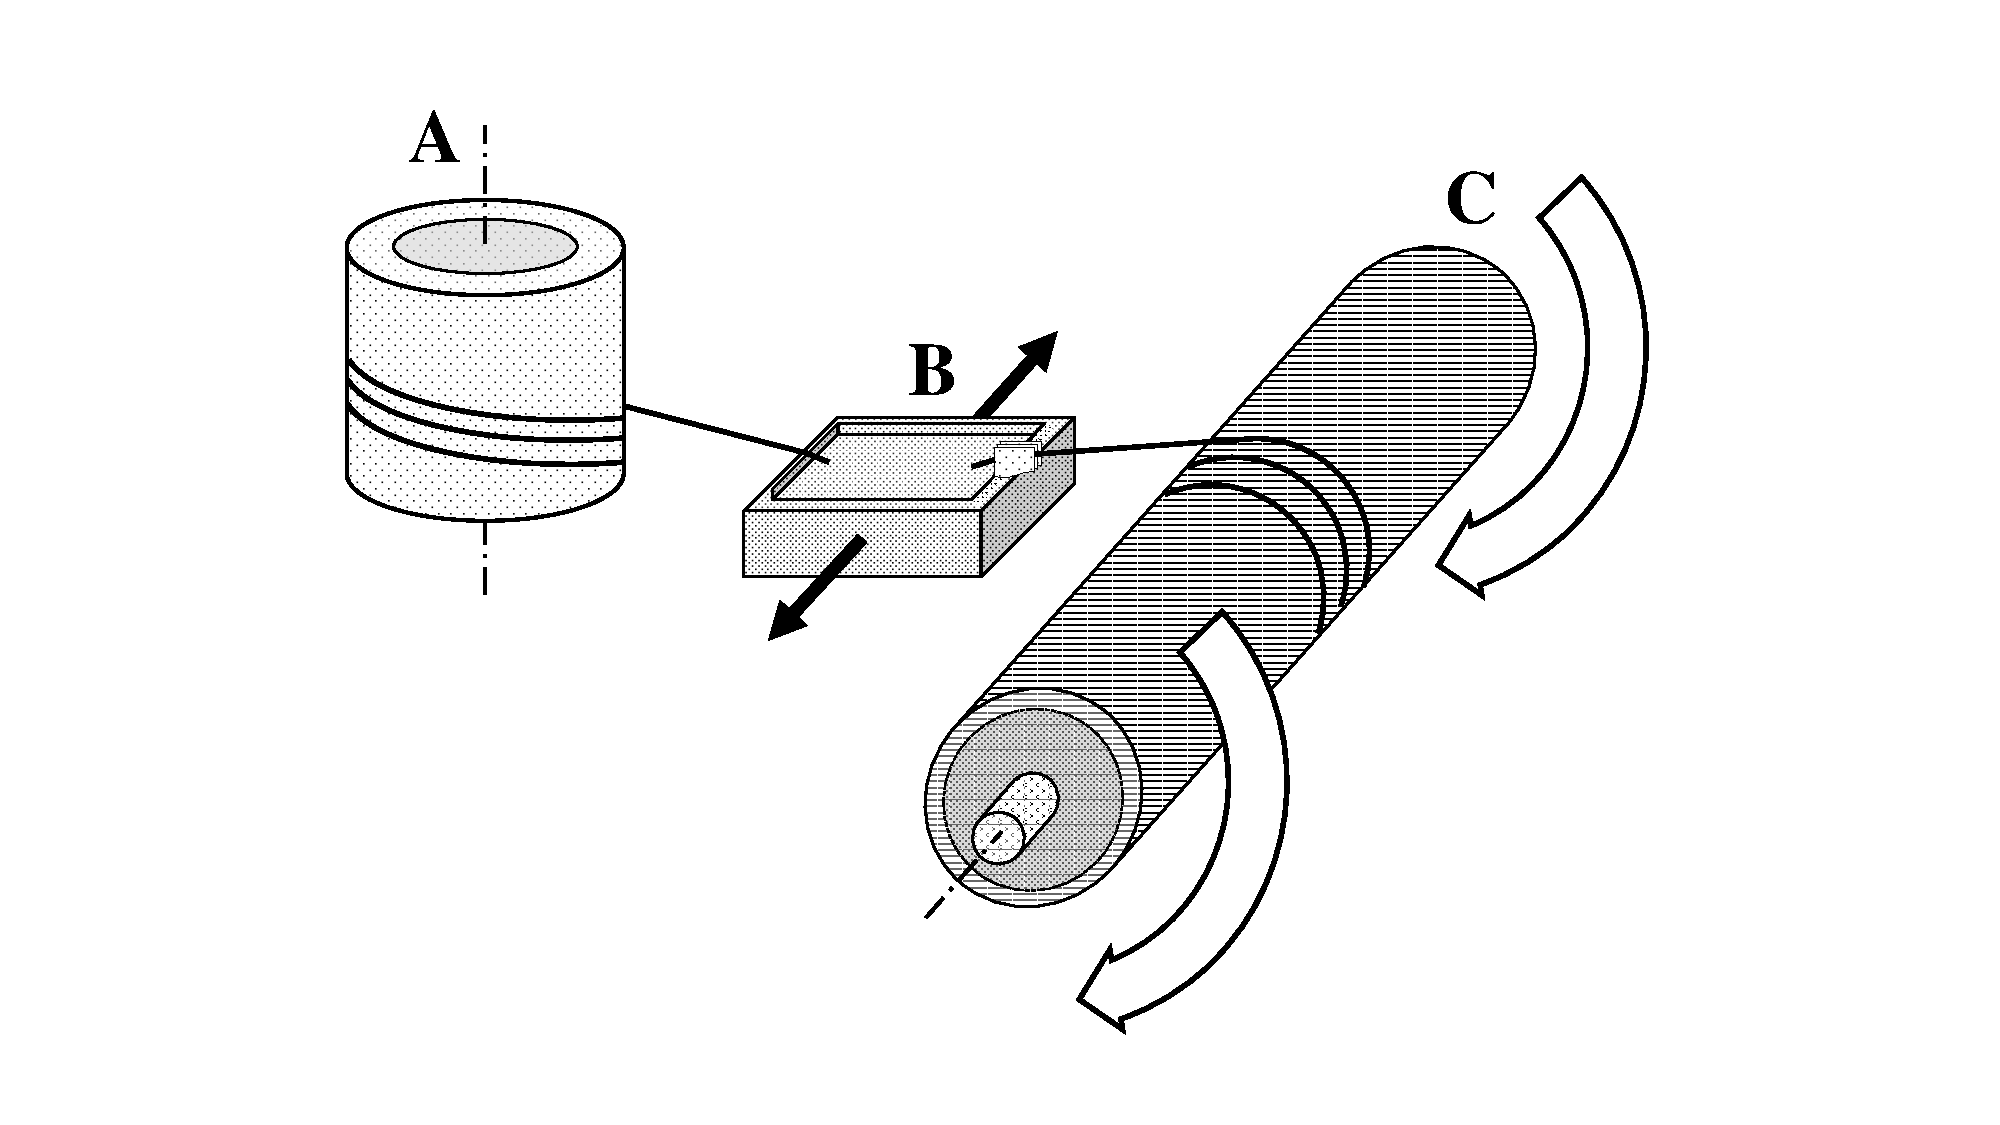
\includegraphics[angle=0, scale=0.45]{imagens/imagem1}
	\caption{Graphical representation of the filament winding machine.}
	\label{i4}
\end{figure}

To geometrically determine the central structure (bench base), the useful winding length was used. Besides this measure, is necessary a relaxation zone, were the winding angle will not be respected. This relaxation zone is important in the moment that the carrier changes direction \citep{livro_prof} and normally it is cut off from the resulting piece. So, to calculate this relaxation zone, it is used the Equation.\ref{e1}:

\begin{equation}\label{e1}
\theta_{min} = arctg \left(\frac{b}{a}\right)
\end{equation}

Where $\theta_{min}$ is the minimum winding angle possible, $b$ is the distance between the eyelet ante the center of the mandrel and $a$ is the relaxation zone. The minimum winding angle chosen for this machine was $33^\circ$, resulting in an relaxation zone of $150 mm$.

Such fact resulted in an mandrel with a total length of $1200mm$. And the structure was developed accordingly, with supports to accommodate such dimensions. The bench base was made even bigger, to let the carrier's eyelet reach the total extension of the mandrel.  



\begin{figure*}[!h]
\centering
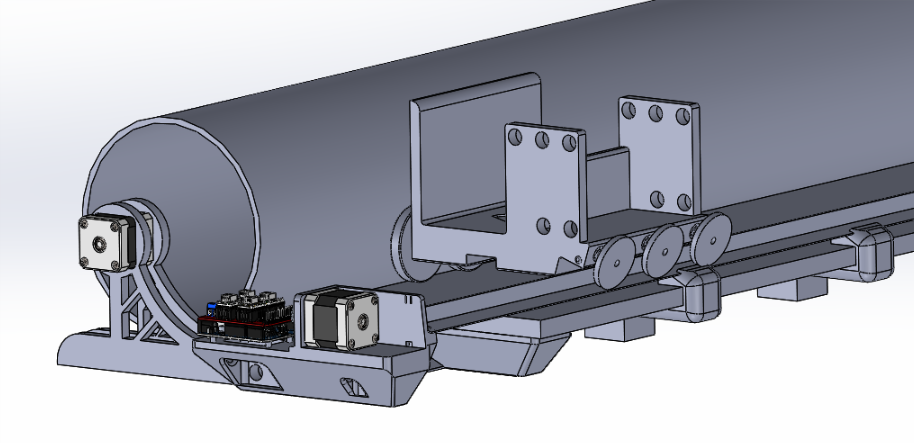
\includegraphics[angle=0, trim = {0mm 0mm 30mm 10mm}, clip , scale=0.3]{imagens/cad}
\caption{Solid Works model design.}
\label{i5}
\end{figure*}




\subsection{ELECTRONIC PARTS}

D) The control system unit:
Breve descriçao das peças eletronicas

citação convniente no topico das partes eletronicas:

The program must control the rotation of the mandrel and how much it must move the carriage in a specific period of time, considering a specific fuselage diameter and length. (PETERS, 2011)


\begin{figure*}[!h]
	\centering
	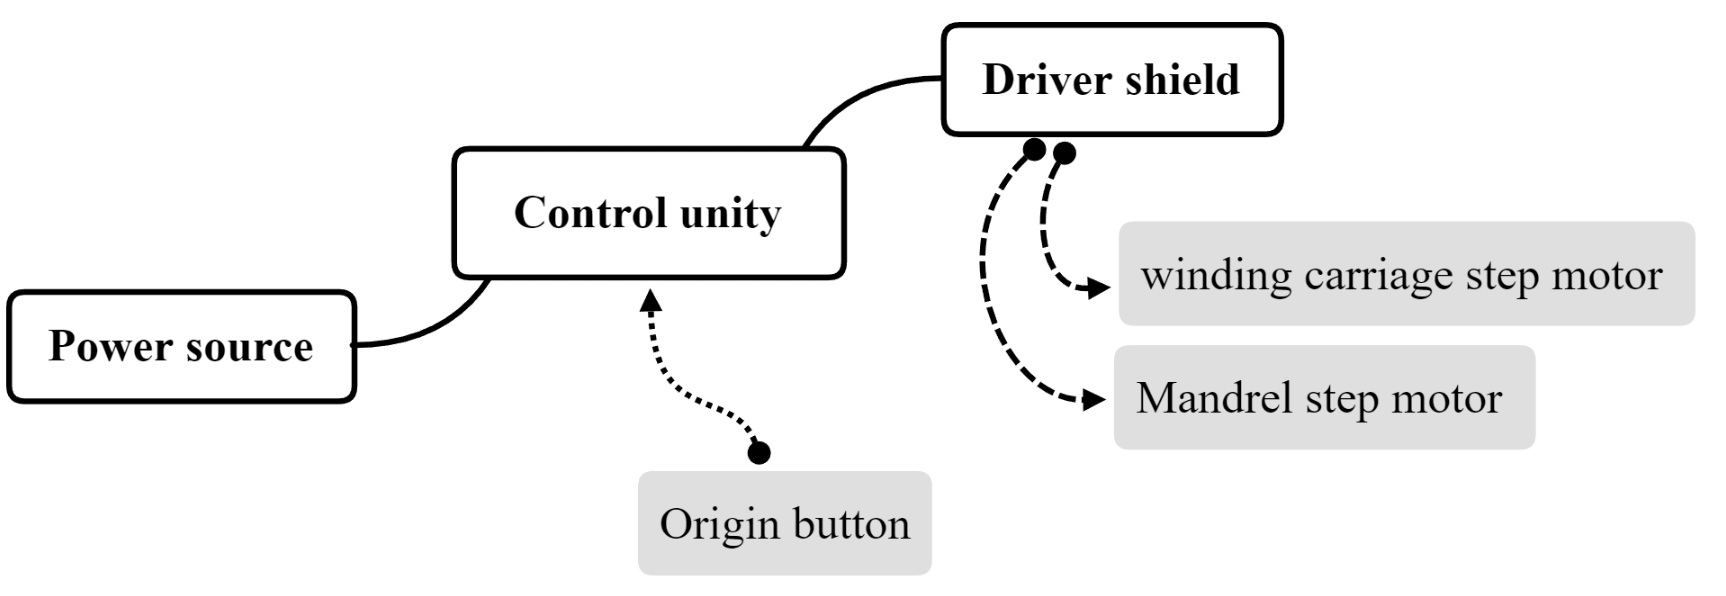
\includegraphics[angle=0, trim = {0mm 0mm 0mm 0mm}, clip , scale=0.25]{imagens/eletronic}
	\caption{Electronic scheme of the controlling unity.}
	\label{i5}
\end{figure*}

\citep{design_fiber} The relation between winding angle and the speed of the screw for mandrel of diameter, This has been calculated using the relations below

\begin{equation}
\theta = \frac{2\pi r N_m}{V_c}
\end{equation}

where $\theta$ is the winding angle, $r$ is the mandrel radius, $N_m$ is the mandrel speed, $v_c$ is the carriage linear velocity.


\begin{equation}
V_c = N_s * d
\end{equation}


where $N_s$ ie the screw speed, $d$ is the screw thread distance.




\section{MECHANISM VALIDATION}
Para a validação da bancada, foram criados tubos de parede fina feitos integralmente de compósitos, para isso, .







\section{ACKNOWLEDGEMENTS}
The authors would like to thank the following professors and institutions: Lmest (Structural Mechanics Laboratory), FEMEC (Mechanical engineering College), UFU (Federal University of Uberl\^andia) and, especially, EPTA(Propulsion and Aerospace Technology Team) for financial support.

\section{REFERENCES} 

\bibliographystyle{abcm}
\renewcommand{\refname}{}
\bibliography{bibfile}

\end{document}
